\chapter{基于局部的特征提取算法}
在上一节的学习过程中,笔者渐渐感觉到计算算子对人脸识别,分类系统的影响非常大,毕竟,人脸图像被分解后,仅仅由一个很短的向量来表示,那该编码系统对样本的区分程度很大程度上就能决定后续分类系统的性能.因此,我渐渐发现了基于局部的特征提取算法,它们有些具有\textit{Content Awareness}的特性,对背景噪声有一定的区分能力,并且可以精细的比较样本的细节之处,因此可以达到精确的识别性能.本章节以SIFT算子为例做介绍.
\subsection{SIFT的原理}
本章节主要基于\cite{lowe2004distinctive, issolah2013sift, juan2009comparison, siftopencv, siftvlfeat, siftubc,lowe1999object}\newline

SIFT算子的计算方法共分4步.
\begin{enumerate}
	\item SIFT首先构建一系列DoG(Difference-of-Gaussian)金字塔.并在其上计算极值,作为该层空间上的特征点.具体的计算方法是求得所有满足在其$3 \times 3$临域上为最大值或最小值的点. 

	 	\begin{center}
		\begin{minipage}[t]{\linewidth}
		%\label{fig:main}
		\center
		{
		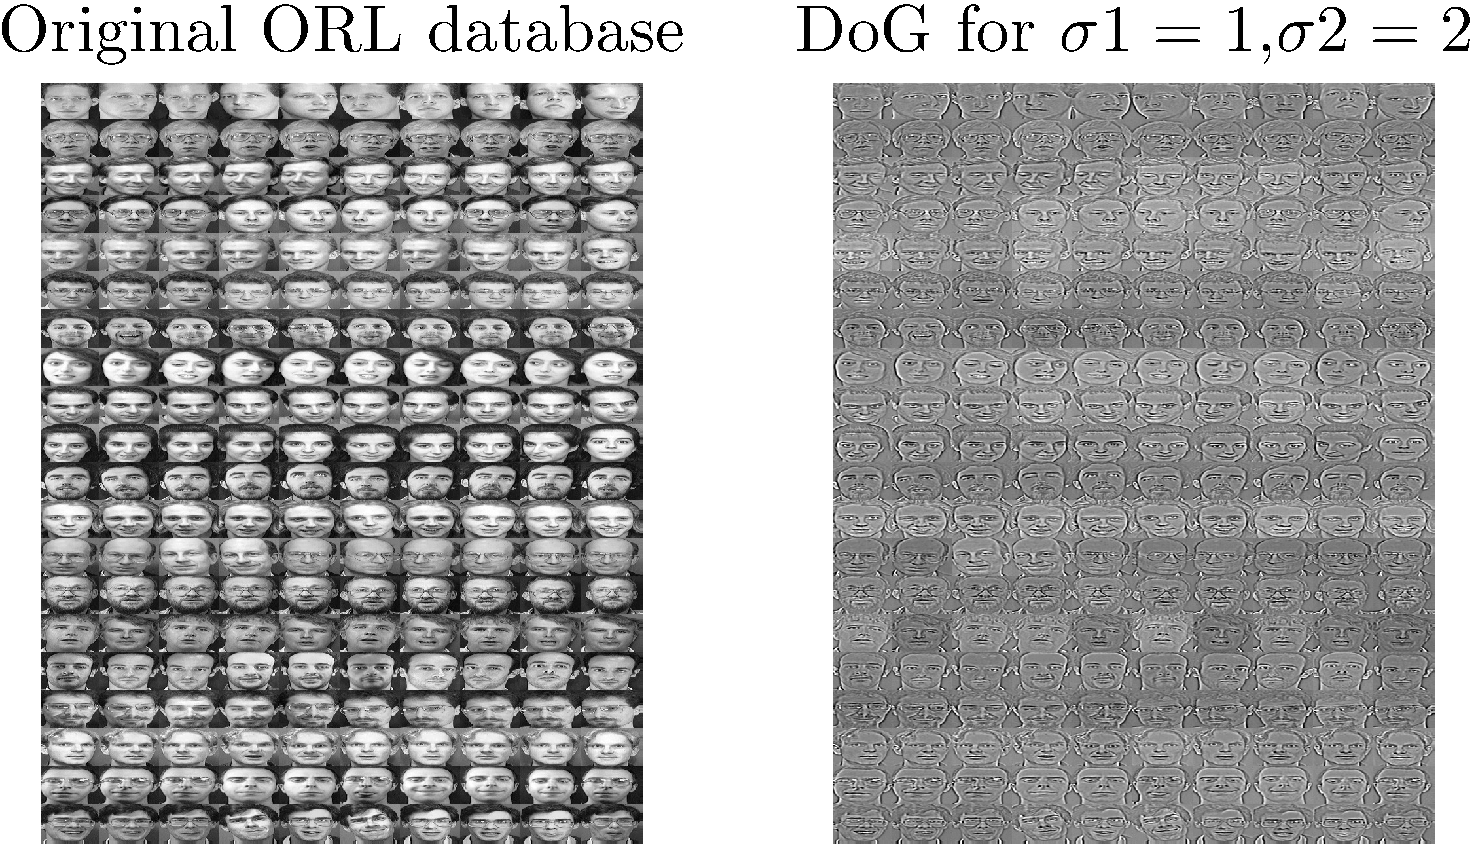
\includegraphics[width=\textwidth]{Img/c3/dog_demo} \captionof{figure}{DoG滤波示意图,DoG图像采用了和输入图像相同的尺度}
		}
		\end{minipage}
		\medskip
		\end{center}
	
	\item 当每层的特征点被计算出来后, SIFT计算该层求得的特征点是否在解析度更大的一层上也满足为最大值或最小值.只有一直满足该特性的点才能被下一步运算.运算结束后,SIFT再一步过滤掉因噪音,边界而被误判为特征点的点.SIFT空间保留了差值运算中特征点相对最初一层邻域的尺度,以及特征点的位置作为特征点的描述.
	\item SIFT在计算出特征位置上每隔$10^\circ$的梯度,并选择梯度最大及三个以内的大于某阈值梯度的方向为该特征位置的方向.经过以上三步,SIFT计算出了输入图片的特征点.
	\item 最后一步是对特征点的描述,SIFT采用一个$N_\theta \times N_x \times N_y$(通常为$8 \times 4 \times 4$,其中$\theta$,$x$,$y$取不同的值,并分别在特征空间上计算梯度)的向量来描述该特征点的性质.在\textit{SIFT-PCA}算法采用了另一种方法.
\end{enumerate}

\subsection{SIFT-PCA算法}
由于SIFT运算结果过长,笔者实现了SIFT-PCA算子\cite{ke2004pca},它是一种采用块压缩技术的基于SIFT的1-3步的方法.具有可调节的长度.

	 	\begin{center}
		\begin{minipage}[t]{\linewidth}
		%\label{fig:main}
		\center
		{
		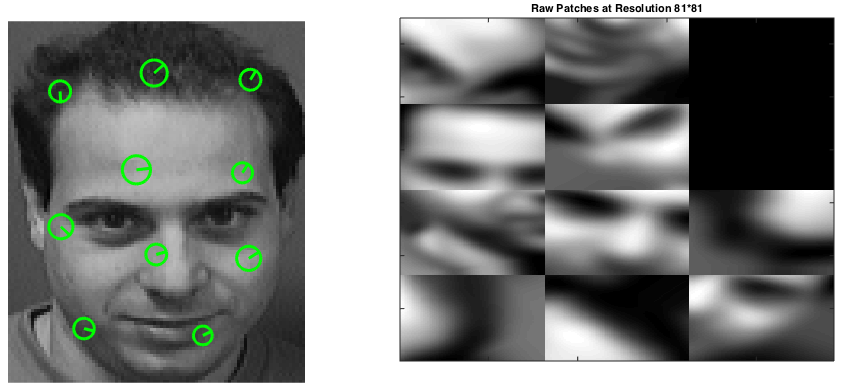
\includegraphics[width=\textwidth]{Img/c3/sift_raw_patch2} 
		\captionsetup{justification=centering}
		\captionof{figure}{SIFT特征点和对应的特征空间示意\\ 为了演示方便,图像中特征点对应$81 \times 81$的邻域,而实际计算中特征点对应$41 \times 41$的邻域}
		}
		\end{minipage}
		\medskip
		\end{center}
	
	它的具体步骤是建立在SIFT算法的1到3步上的,在标准特征位置所描述的空间上:
	\begin{enumerate}
		\item SIFT-PCA算法首先计算该空间的水平,竖直两个梯度空间(本文中使用了Sobel方法)
			
		\begin{center}
		\begin{minipage}[t]{\linewidth}
		%\label{fig:main}
		\center
		{
		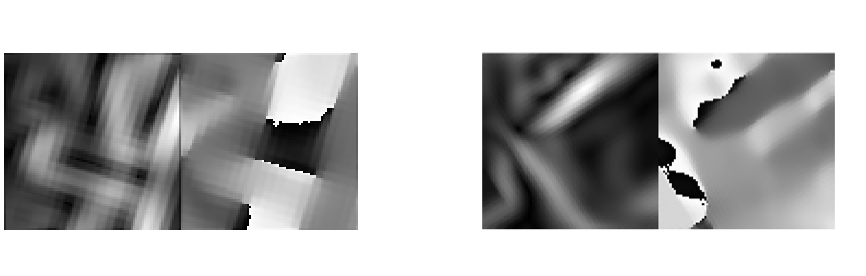
\includegraphics[width=\textwidth]{Img/c3/gradient.png} 
		\captionsetup{justification=centering}
		\captionof{figure}{水平,竖直两个梯度空间示意\\ 左:使用Sobel算子,右:使用prewitt算子}
		}
		\end{minipage}
		\medskip
		\end{center}
		
		\item SIFT-PCA计算多张图片多个特征点上的梯度空间,并且使用PCA对其进行降维运算
		\item 当新输入空间时,SIFT-PCA使用标准SIFT算法提取特征点及特征点对应的空间,计算出对应空间的水平,竖直梯度空间后,对这两个空间使用上一步的基底降维.坐标就是SIFT-PCA对特征点对应的描述
	\end{enumerate}
	本文实现中,使用了100个人所提取出的特征梯度空间用作SIFT-PCA基底的学习,并在3600左右的特征向量中取前20个作为PCA降维后的特征向量,降维后的前20特征值占据了约50\%的特征值,下面是PCA的特征值绘制:
	
			\begin{center}
		\begin{minipage}[t]{\linewidth}
		%\label{fig:main}
		\center
		{
		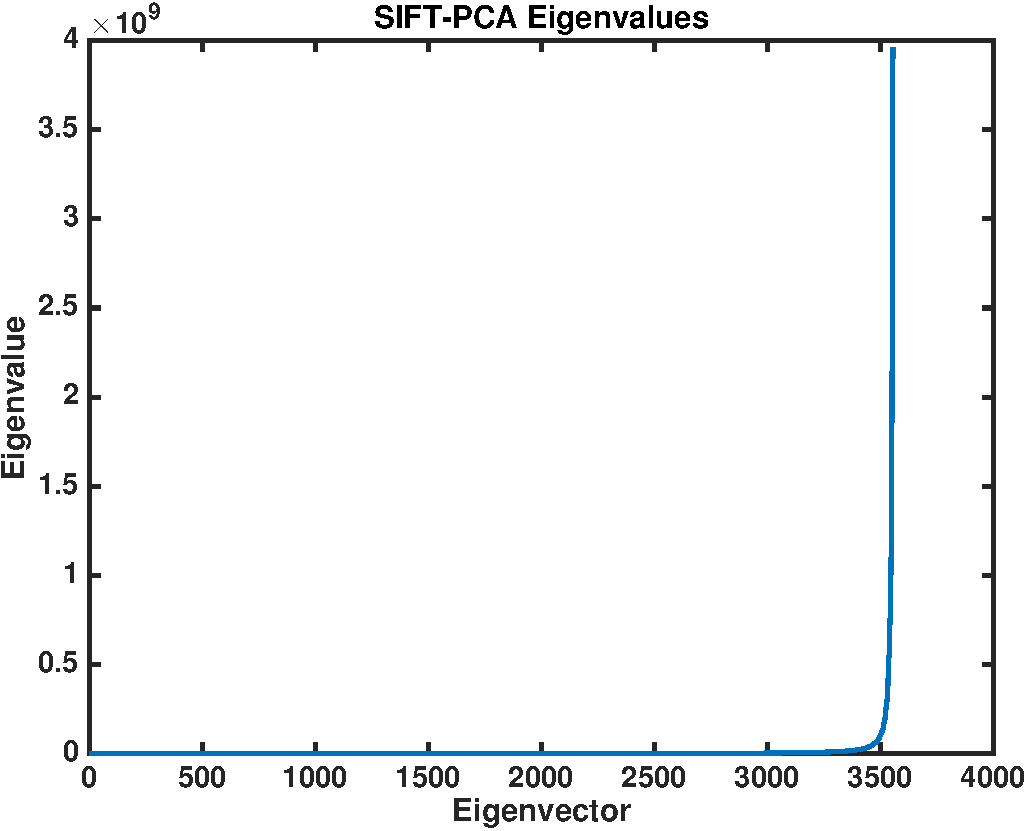
\includegraphics[width=\textwidth]{Img/c3/sift_pca_eigen} 
		\captionof{figure}{PCA的特征值}
		}
		\end{minipage}
		\medskip
		\end{center}
		
		

\subsection{SIFT的编码方法}
由于SIFT算子是\textit{Content Aware}的,其特征提取的结果是由若干个提取位置上的描述子来描述的,因此,长度并不固定.这对后续的分类算法并不友好.因此,SIFT的结果大都被编码了,编码方法通常有以下的方法.\cite{chatfield2011devil}

\subsection{NBNN分类法}
由于SIFT的特性,本项目在上一节固定编码的同时,也结合SIFT特性实现了简单的NBNN算法.NBNN算法不需要对SIFT进行特殊的编码,同时可以并行运算.并且结果也很好.